\section{Supplementary Materials for Section~\ref{sec:experiments}}
\label{sec:supp-to-experiment}
The three-class data we used in Section~\ref{sec:experiments} is originally generated in a $d=2$ plate as shown in the following figure: 
\begin{figure}[h]
    \centering
    \begin{subfigure}[b]{0.23\textwidth}  
        \captionsetup{justification=centering}
        \begin{center}
        \hspace*{-0.3cm} 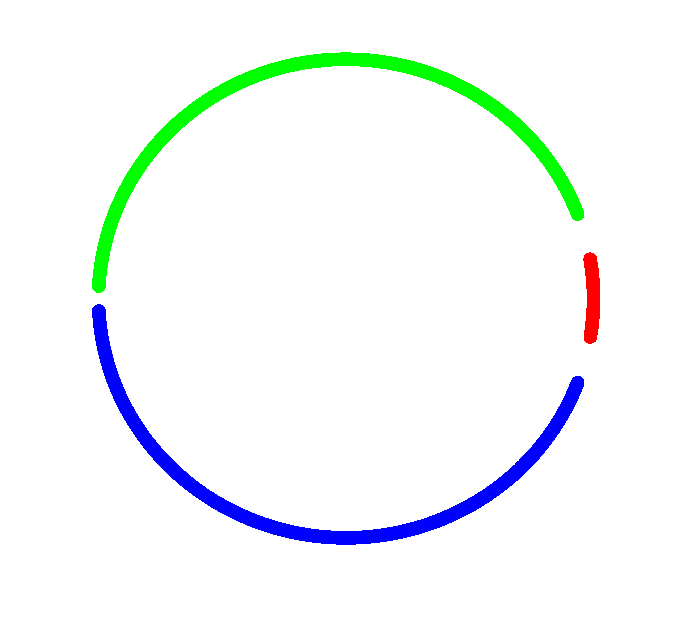
\includegraphics[width=1.15\textwidth, trim={0, 0cm, 0, 0}, clip]{figures/strong_points}
        \caption{Strongly separable case}
        \label{fig:strong-points}
        \end{center}
    \end{subfigure}
    \hfill
    \begin{subfigure}[b]{0.23\textwidth} 
        \captionsetup{justification=centering}
        \centering
        \hspace*{-0.3cm}  
\includegraphics[width=1.15\textwidth, trim={0, 0cm, 0, 0}, clip]{figures/weak_points}
         \caption{Weakly separable case}
    \end{subfigure}
    \vspace*{-0.2cm}
    \caption{Data distribution for Section~\ref{sec:experiments}}
    % \caption{Comparison between our algorithm and Banditron with different exploration parameter $\epsilon$ under $\gamma=0.05$ and $K=3$. }
\end{figure}

However, in 2D, the samples in Figure~\ref{fig:strong-points} do not satisfy the strong linear separability defined in Definition~\ref{definition:weak-linear-separability}, which requires that any class can be separated from all the others by a hyperplane that \textit{passes through the origin}. We therefore raise the dimensionality to 3D by adding a constant feature to all samples. This is equivalent to allowing the separating hyperplanes to have a bias, so that they do not need to pass through the origin. Thus Figure~\ref{fig:strong-points} becomes strongly linearly separable. To better understand how each algorithm works, we plot below the final decision boundary that is learned by each algorithm. 

\begin{figure}[h!]
    \centering
    \begin{subfigure}[b]{0.23\textwidth}  
        \captionsetup{justification=centering}
        \begin{center}
        \hspace*{-0.3cm} 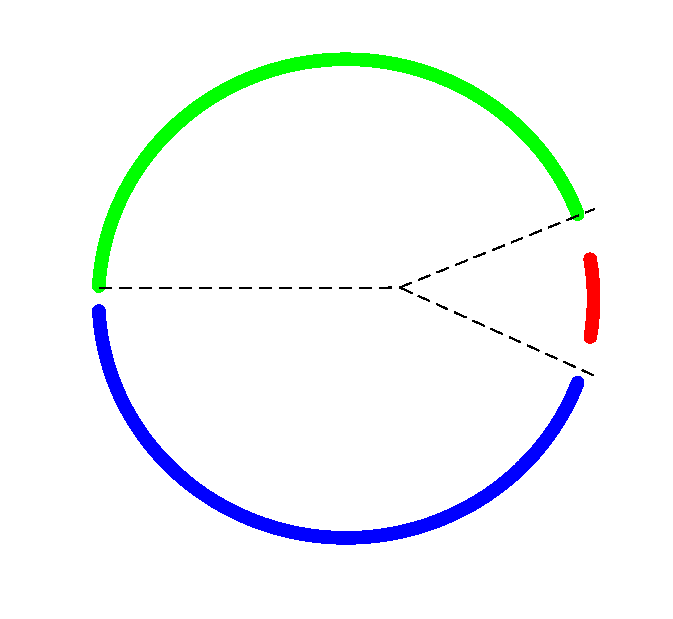
\includegraphics[width=1.15\textwidth, trim={0, 0cm, 0, 0}, clip]{figures/strong_banditron_points}
        \caption{Strongly separable case}
        \label{fig:strong-points}
        \end{center}
    \end{subfigure}
    \hfill
    \begin{subfigure}[b]{0.23\textwidth} 
        \captionsetup{justification=centering}
        \centering
        \hspace*{-0.3cm}  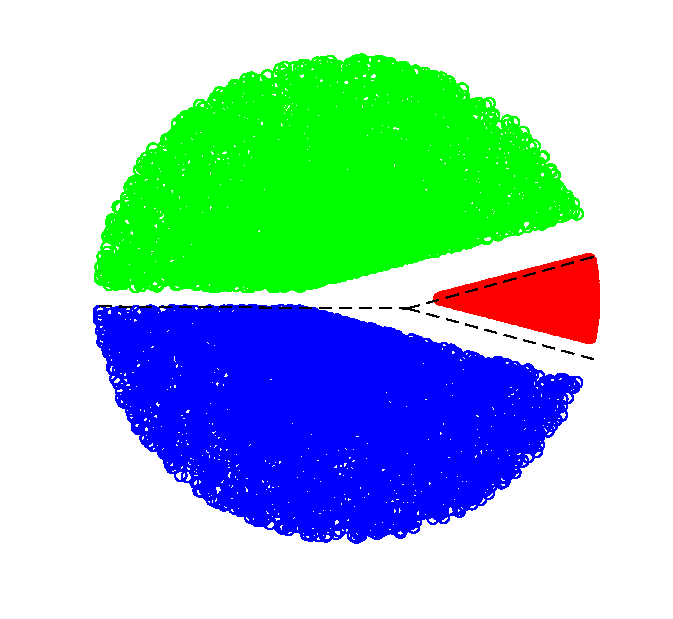
\includegraphics[width=1.15\textwidth, trim={0, 0cm, 0, 0}, clip]{figures/weak_banditron_points}
         \caption{Weakly separable case}
    \end{subfigure}
    \vspace*{-0.2cm}
    \caption{\textsc{Banditron}'s decision boundary}
    % \caption{Comparison between our algorithm and Banditron with different exploration parameter $\epsilon$ under $\gamma=0.05$ and $K=3$. }
\end{figure}

\begin{figure}[h!]
    \centering
    \begin{subfigure}[b]{0.23\textwidth}  
        \captionsetup{justification=centering}
        \begin{center}
        \hspace*{-0.3cm} 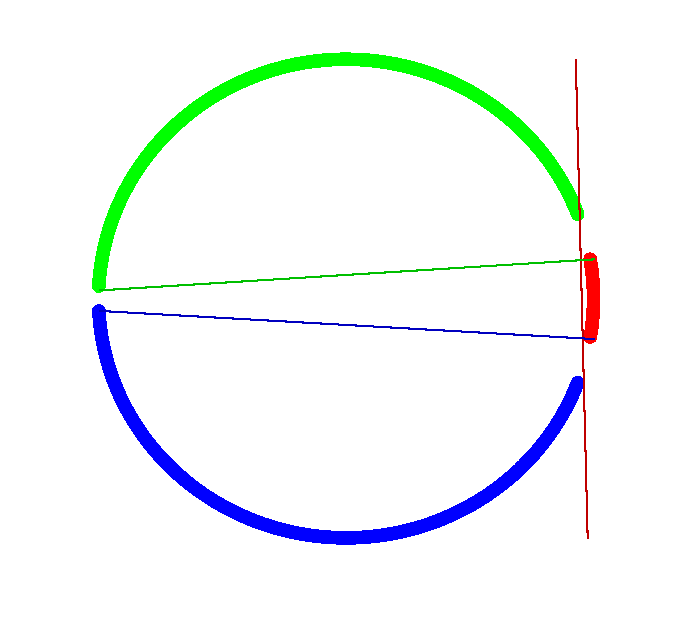
\includegraphics[width=1.15\textwidth, trim={0, 0cm, 0, 0}, clip]{figures/strong_linear_ova_points}
        \caption{Strongly separable case}
        \label{fig:strong-points}
        \end{center}
    \end{subfigure}
    \hfill
    \begin{subfigure}[b]{0.23\textwidth} 
        \captionsetup{justification=centering}
        \centering
        \hspace*{-0.3cm}  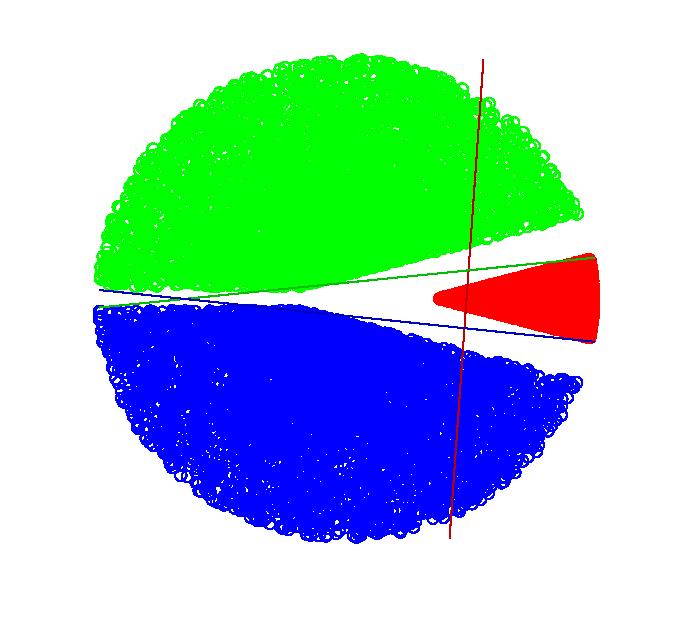
\includegraphics[width=1.15\textwidth, trim={0, 0cm, 0, 0}, clip]{figures/weak_linear_ova_points}
         \caption{Weakly separable case}
    \end{subfigure}
    \vspace*{-0.2cm}
    \caption{Our Algorithm with linear kernel (Algorithm~\ref{algorithm:algorithm-for-strongly-linearly-separable-examples})'s decision boundary}
    % \caption{Comparison between our algorithm and Banditron with different exploration parameter $\epsilon$ under $\gamma=0.05$ and $K=3$. }
\end{figure}

\begin{figure}[h!]
    \centering
    \begin{subfigure}[b]{0.23\textwidth}  
        \captionsetup{justification=centering}
        \begin{center}
        \hspace*{-0.3cm} 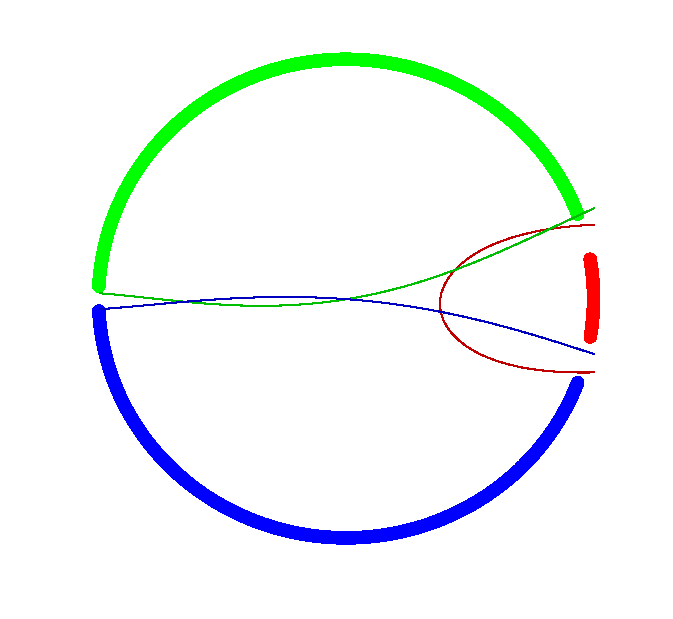
\includegraphics[width=1.15\textwidth, trim={0, 0cm, 0, 0}, clip]{figures/strong_rational_ova_points}
        \caption{Strongly separable case}
        \label{fig:strong-points}
        \end{center}
    \end{subfigure}
    \hfill
    \begin{subfigure}[b]{0.23\textwidth} 
        \captionsetup{justification=centering}
        \centering
        \hspace*{-0.3cm}  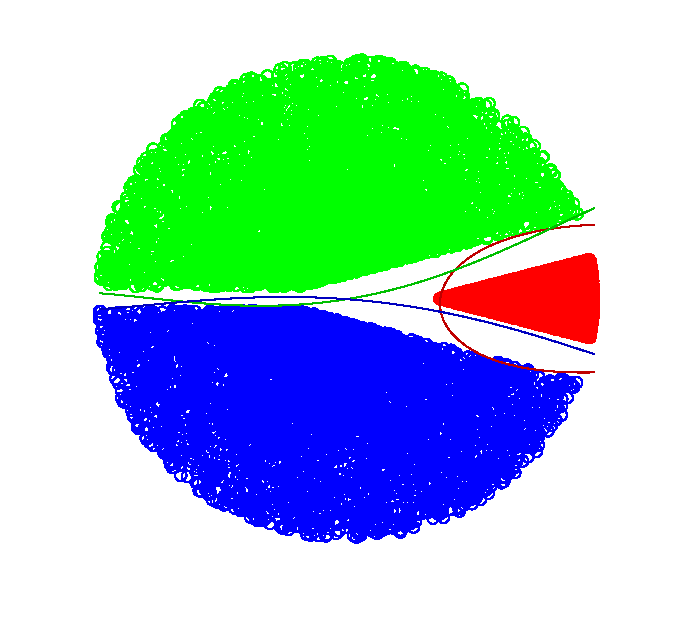
\includegraphics[width=1.15\textwidth, trim={0, 0cm, 0, 0}, clip]{figures/weak_rational_ova_points}
         \caption{Weakly separable case}
    \end{subfigure}
    \vspace*{-0.2cm}
    \caption{Our Algorithm with rational kernel (Algorithm~\ref{algorithm:kernelized})'s decision boundary}
    % \caption{Comparison between our algorithm and Banditron with different exploration parameter $\epsilon$ under $\gamma=0.05$ and $K=3$. }
\end{figure}

